\chapter{Introduction}
\label{intro}
Datagram Transport Layer Security (DTLS)\cite{rescorla2006datagram} is a well-known security protocol that provides security on top of User Datagram Protocol (UDP) transport layer communications. It is explicitly designed to be as similar to as possible to Transport Layer Security (TLS)\cite{rescorla2018transport}, which operates on top of Transmission Control Protocol (TCP) and provide similar level of security guarantees, that is, certificate-based authentication, confidentiality and integrity of data exchanged to allow communications between client/server applications without eavesdropping, unauthorized accesses, or message tampering, while preserving datagram semantics of the underlying transport protocol. As a datagram protocol, DTLS doesn't guarantee the reliability or order of packet delivery. Unlike TLS, DTLS is resilient in the face of invalid or lost in transmission of records (e.g., invalid formatting, length, MAC, etc.) by silently discarding invalid packets, thus preserving the session. This makes it suitable for securing real-time applications and services that are delay-sensitive (and hence use datagram transport) such as online gaming, live streaming, Internet telephony, tunneling applications such as VPNs, and applications that tend to run out of file descriptors or socket buffers. Currently, it is one of the primary protocols for securing IoT applications such as Constrained Application Protocol(CoAP). DTLS is also used as one of the two security protocols in WebRTC, a framework enabling real-time communication, to implement video conferencing in browsers without the need for a plugin.

Currently, designers of these applications are faced with unsatisfactory choice like IPsec\cite{kent1998rfc2401IPSEC} that is composed of a number of different pieces to provide confidentiality, integrity, and replay protection, or custom application layer security protocol which typically require a large amount of effort to design. DTLS is designed to run in application space and doesn’t need any kernel modifications and hence is more practical approach.

TESLA\cite{perrig2002tesla}, proposed by Perrig et al. in 2002, provides delayed per-packet data authentication and source authentication, to secure lossy broadcast communication. The key idea to provide both efficiency and security is a delayed disclosure of keys, which results in an authentication delay. At a high level TESLA uses a new MAC key for each packet, which will be sent by the sender after sufficient delay, that ensures the key will not be captured by a network attacker. The MAC keys are hash chain of keys and revealed in opposite direction of generation, hence finding next key depends n reversing the hash algorithm. The receiver can verify integrity of a received packet only after it receives the key in a later packet. The first key is signed with a digital signature to provide source authentication. It has been shown that security of TESLA depends on knowing a bound on the time discrepancy of the sender and the receiver's clock, and not the network delay.

\begin{figure}[H]
    \centering
    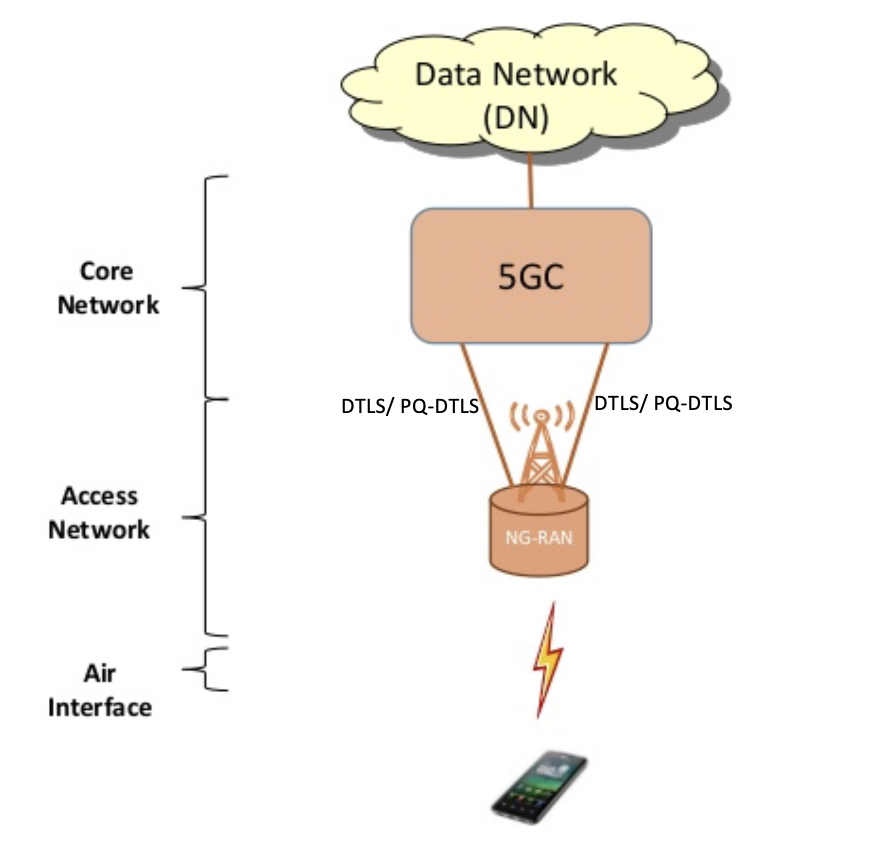
\includegraphics[height=5cm,width=7.5cm]{figures/5g-cn-ran.png}
    \caption{Application of DTLS/PQ-DTLS for securing communication between Radio Access Network(NG-RAN) and Core Network(5GC)}
    \label{5g-cn-ran}
\end{figure}


The development of quantum computer, will pose a threat to current public key algorithms, such as RSA and ECC. Therefore, the National Security Agency(NSA)\cite{NSA}, has issued a statement recommending to transition to Quantum-Safe cryptography in near future. NSA suggests in \cite{NSAonPQ} that existing cryptography may remain secure for a while even after the quantum computing era properly arrives, perhaps giving us enough time to update it.


The application of DTLS, as additional, underlying security protocol, has been proposed by 5G security architecture \cite{huawei5g} to secure signaling transmission on the control plane\footnote{Control plane refers to all the functions and processes that determine which path to use. Routing protocols, spanning tree, ldp, etc are examples.}, ensuring transport security between radio access networks(RANs) and core networks (See fig. \ref{5g-cn-ran}). The communication between NG-RANs and 5GC essentially requires two security properties : data integrity and origin authentication of signaling data. The integrity of signaling data is mandatory and provides protection against rogue BS attacks\footnote{A rogue BS is a malicious station that impersonates a legitimate access point  (AP).  The  rogue  BS  attack  represents  a  major  denial-of-service  threat  against  wireless  networks.}  and origin authentication is required to verify that signal comes from a intended source.\cite{boudriga2009security}

\textbf{Problem.}
There are several use cases in which communications privacy is not strictly needed, although authenticity of the communications transport is still very important.

While TESLA provides lightweight source authentication and data integrity, the direct replacement of TESLA algorithms with their post-quantum version will add to the processing and communication cost. However existing DTLS versions do not provide support for post-quantum security for data stream authentication. 

\textbf{Solution.} 
As all cryptographic primitives TESLA uses have post-quantum security, except the signature scheme, we replace it with a hash-based signature to construct a post-quantum version, and call it PQ-TESLA. This scheme assure source authentication and data integrity against quantum computers. We design a ready-to-use protocol by integrating PQ-TESLA in existing DTLS, thus, creating a post-quantum DTLS for source authentication and data integrity.

We provide novel and standard compliant post-quantum DTLS mechanisms that aims to increase the applicability of DTLS for post-quantum applications. Most importantly, our proposed PQ-DTLS does not compromise the end-to-end security properties provided by DTLS. 

 
\section{Contributions}
Our contributions is two-fold which includes design and implementation of (1) PQ TESLA for authentication and integrity for streams (2) PQ-DTLS with source authentication and integrity only, which is application PQ-TESLA to DTLS. 

We limit ourselves to providing post-quantum security for origin  authentication and message integrity to DTLS. A post-quantum version of DTLS, maintains security guarantees of of DTLS and can be efficiently implemented. 

We use existing lightweight stream authentication protocol, TESLA proposed by \cite{perrig2000efficient}, which consists of only hash functions and one digital signature. We implement a post-quantum version of TESLA, PQ-TESLA, by just replacing signature scheme with a hash-based signature algorithm, K2SN-MSS \cite{karati2019k2sn}. We provide PQ-DTLS design, by modifications to existing DTLS protocol with additional PQ-TESLA components. We also, provide an efficient implementation of PQ-DTLS with source authentication and integrity, by application of PQ-TESLA to DTLS.


\textcolor{red}{Our work can be extended to provide post-quantum confidentiality as well.}

Our PQ-DTLS modifies two handshake messages of DTLS to ensure the required initialization information of TESLA (timing information) are exchanged. The additional initialization messages contain time synchronization and key disclosure details, hence, are signed by K2SN signature that provides origin authentication, while the integrity of record layer packets are based on traditional TESLA per packet key disclosure. The handshake messages of DTLS are shown in Figure \ref{dtls(auth)} and modified DTLS handshake messages in figure \ref{hs-dtls_tesla1}, where the modified flights are shown in \textcolor{red}{red}.

\subsection{Implementation \& Evaluation} We use dtls library TinyDTLS\cite{} and modify the handshake layer and record layer to integrate PQ TESLA, which results in PQ DTLS with source authentication and message integrity.


For evaluation of our integrated PQ TESLA into DTLS, we show the feasibility of our integrated scheme. We also evaluate them based on overhead involved, cryptographic primitives used and time consumption, using one existing signature scheme(ECDSA) and a hash based signature scheme(K2SN-MSS \cite{karati2019k2sn}). We show the cost of integrating post-quantum security to DTLS with source authenticity and integrity, hence we use ECDSA signature. The implementation of client(aka sender) and server(aka receiver) is facilitated by employing the socket API programming interface.

Suggested performance metrics that are suitable for our implementation are below:
\begin{enumerate}
    \item Evaluation of cryptographic primitives : Run-time for Key Generation, Signature Generation and Verification functions of ECDSA and K2SN-MSS signature schemes.
    \item Packet overhead - Handshake packet overhead and Application data packet Overhead - for DTLS, DTLS-TESLA,PQ-DTLS-TESLA.
    \item Handshake latency for DTLS, DTLS-TESLA, PQ-DTLS-TESLA.
    \item Application Data transfer latency : Payload size versus time consumed by DTLS, DTLS-TESLA,PQ-DTLS-TESLA.
    \item Memory Usage and code-size of the implementated source code.
    % \item Speed and communication size of request and response of TESLA.
\end{enumerate}{}


We also provide security analysis of PQ-TESLA and PQ-DTLS scheme and claim that it is secure against quantum computers. We also, claim that the integration of PQ TESLA in DTLS, does not lower security guarantees provided by classical DTLS protocol. 

\textcolor{red}{The sharing of public key between sender and receiver is out of scope of our work, we discuss briefly usage of raw public keys or pre-shared key.}\ref{}





\section{Thesis Organization }
Section \ref{Preliminaries} provides the necessary detailed background on TESLA protocol, K2SN-MSS signature scheme and DTLS protocol. An overview of related work is discussed in section \ref{relatedwork}. Section \ref{PQIntegration} describes the integration of PQ security to TESLA and its application to DTLS library, called, tinyDTLS. We also provide the security analysis in section \ref{SecurityAnalysis}.

The experiments and evaluation of resultant implementation of the PQ scheme is discussed in section \ref{Evaluation}.\\